% ============================================================
% CHAPITRE 2 : MÉTHODOLOGIE & ARCHITECTURE
% ============================================================
\chapter{Méthodologie et architecture}
\label{ch:methodo}

\section{Architecture générale du pipeline hybride}

L'architecture d'\AZIZA repose sur le principe fondamental de \textbf{séparation stricte des préoccupations} : la forme et le fond sont évalués par des modules indépendants, garantissant que les hallucinations potentielles du LLM n'affectent jamais les critères quantitatifs.

\begin{figure}[h]
\centering
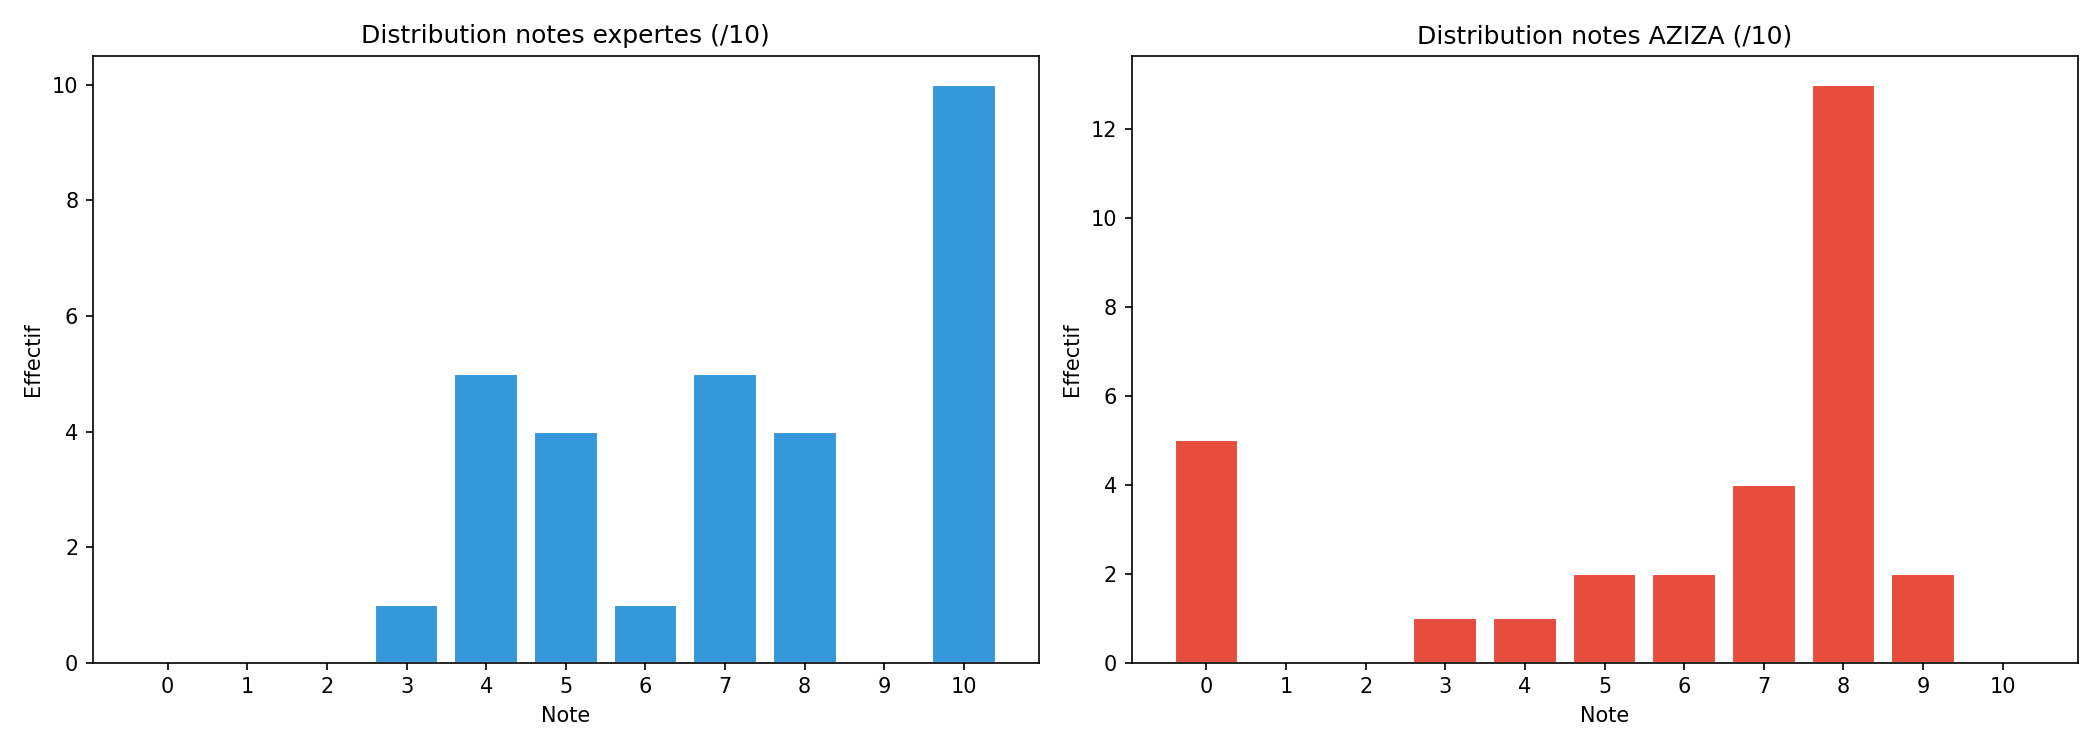
\includegraphics[width=\textwidth]{distribution_comparee.png}
\caption{Architecture générale du pipeline AZIZA}
\label{fig:architecture}
\end{figure}

\subsection{Couche déterministe — Forme (/7)}

La couche \textbf{Forme} utilise exclusivement des algorithmes déterministes :

\begin{itemize}
    \item \textbf{Lexical (/3)} : calcul du LCS (Longest Common Subsequence) normalisé entre le texte source et la contraction, transformé via une fonction parabolique avec paramètres \(S_{\min}=0.26\) et \(S_{\max}=0.80\). Une pénalité de quota continue est appliquée : \(\min(2, \text{écart\_pct}/50)\).
    \item \textbf{Syntaxe (/2)} : ratio du nombre de phrases entre la source et la contraction, combiné à une analyse des connecteurs logiques (9 catégories : addition, opposition, cause, conséquence, illustration, concession, conclusion, temporalité, condition).
    \item \textbf{Orthographe (/2)} : via l'API LanguageTool en mode distant, avec un barème dégressif multiplié par \(\min(1, \text{nb\_mots}/30)\).
\end{itemize}

\subsection{Couche sémantique — Fond (/3)}

La couche \textbf{Fond} fait appel au LLM Mistral Small dans un cadre strictement borné :

\begin{enumerate}
    \item \textbf{Embedding sémantique} : calcul de la similarité cosinus entre les embeddings du texte source et de la contraction via \texttt{mistral-embed}.
    \item \textbf{LLM Few-Shot + CoT} : le modèle reçoit 5 exemples (Few-Shot) et doit suivre une chaîne de pensée obligatoire avant de produire un score /3, une détection de contresens, une détection de subjectivité, un diagnostic d'erreur, un micro-cours, et un exemple de reformulation.
    \item \textbf{Calibration hybride} : fusion du score LLM et du score de similarité sémantique avec correction des écarts.
\end{enumerate}

\section{Machine à états de l'apprenant}

\AZIZA implémente une \textbf{machine à états à 3 paliers} pour modéliser la progression :

\[
M_p = 0.4 \times \text{moyenne des exercices} + 0.6 \times \text{note du test de niveau}
\]

\begin{itemize}
    \item \textbf{Palier 1 — Découverte} : premier contact avec la contraction, exercices guidés.
    \item \textbf{Palier 2 — Consolidation} : renforcement des compétences acquises.
    \item \textbf{Palier 3 — Maîtrise} : autonomie complète, textes complexes.
\end{itemize}

Les seuils de passage sont calibrés à 75\% du maximum pour le passage au palier supérieur.

\section{Génération du corpus d'expérimentation}

Pour constituer le corpus de 30 contractions, nous avons développé un \textbf{système de prompts contrôlés} garantissant une répartition équilibrée :

\begin{itemize}
    \item \textbf{10 contractions correctes} : reformulation complète, quota respecté, toutes les idées présentes.
    \item \textbf{10 contractions partiellement correctes} : avec un défaut (léger hors quota, contresens mineur, similarité légère, omission d'idée).
    \item \textbf{10 contractions incorrectes} : avec un défaut grave (plagiat manifeste, contresens majeur, hors quota grave).
\end{itemize}

Chaque génération utilise un prompt système fixe définissant les règles officielles du BAC béninois et un prompt utilisateur variable spécifiant le texte source et le type de défaut à injecter.

\section{Verrous pédagogiques}

Quatre verrous éliminatoires protègent l'intégrité de l'évaluation :

\begin{itemize}
    \item \textbf{Plagiat} (LCS \(\geq 0.80\)) : note globale = 0/10.
    \item \textbf{Hors-sujet} (similarité sémantique < 0.85) : fond = 0/3, pénalité forme = \(-1\) pt.
    \item \textbf{Texte trop court} (nb mots < 20) : note globale = 0/10.
    \item \textbf{Subjectivité} (pronoms personnels, expressions d'opinion) : fond \(-1\) pt.
\end{itemize}

\section{Évolution de l'architecture : de v1.0 à v2.0}

Le passage de la version 1.0 (spécifiée dans le cahier des charges) à la version 2.0 a introduit plusieurs améliorations majeures :

\begin{itemize}
    \item \textbf{API REST complète} avec authentification par clé (`X-API-Key`) et rate limiting (60 requêtes/min).
    \item \textbf{Documentation Swagger} interactive (8 endpoints documentés).
    \item \textbf{Augmentation des tests} : de 110 à 117 tests unitaires.
    \item \textbf{Format `content` en tableau de parties} pour la compatibilité avec l'API Mistral 2026.
    \item \textbf{Déploiement PythonAnywhere} remplaçant Docker suite aux changements de politique de HuggingFace Spaces.
\end{itemize}
